\documentclass[10pt]{beamer}

\usetheme[progressbar=frametitle]{metropolis}
\usepackage{appendixnumberbeamer}
\usepackage{amssymb}
\usepackage{amsmath}
\usepackage{booktabs}
\usepackage[scale=2]{ccicons}
\usepackage{tikz}
\usepackage{relsize}
\usepackage{pgfplots}
\usepackage[colorlinks]{hyperref}
\usepgfplotslibrary{dateplot}
\usepackage{wrapfig}
\usepackage{xspace}
\newcommand{\themename}{\textbf{\textsc{metropolis}}\xspace}

\usepackage{graphicx}

\usepackage{subcaption}

\usepackage[export]{adjustbox}
\title{EE5606 : Convex Optimization}
% \date{\today}
\date{}
\author{Srujana B - MA17BTECH11001 \newline Nikhil Gandi - MA17BTECH11002 \newline Vyshnavi - MA17BTECH11005 \newline Venkata Datta Sai - MA17BTECH11007 \newline Aravind Reddy K V - MA17BTECH11010}
\institute{Mathematics and Computing, IIT-Hyderabad}
% \titlegraphic{\hfill\includegraphics[height=1.5cm]{logo.pdf}}
\begin{document}
\maketitle

\section{Newton's Method and it's Variants}
\begin{frame}[fragile]{Newton's Method}
The classic Newton-Raphson method for root finding is : \newline
\begin{center}
    $\boldsymbol{x_{n+1} = x_n - \frac{f(x_n)}{f'(x_n)}}$
\end{center}
This method approximates $f(x)$ to be \textbf{linear} at $x_n$ and finds the root of that function. This root is our new $x_n$.
\begin{center}
    \graphicspath{ {./images/} }
    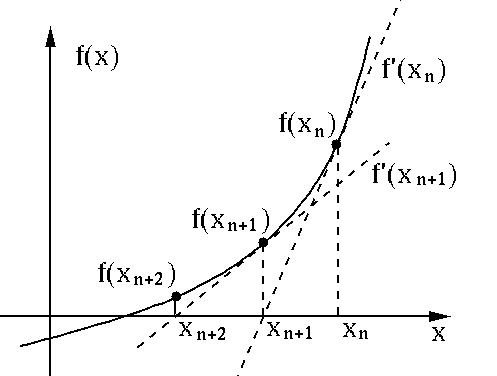
\includegraphics [scale=0.35] {NR}
\end{center}
\end{frame}

\begin{frame}[fragile]{Newton's Method in Optimization}
 \begin{itemize}
     \item In optimization, we look for minimum or maximum of an objective function.
     \vspace{3mm}
     \item This can be obtained by setting derivative of objective function to 0. So, we are interested in finding roots of $\boldsymbol{f'(x)=0}$. 
      \vspace{3mm}
     \item This can be found by using the previously discussed Newton-Raphson Method to $f'(x)$ instead of $f(x)$.
   \end{itemize}
Hence, our iterative scheme changes to the following : \newline
\begin{center}
    $\boldsymbol{x_{n+1} = x_n - \frac{f'(x_n)}{f''(x_n)}}$ 
\end{center}
\end{frame}

\begin{frame}[fragile]{Newton's Method in Optimization}
 \textbf{Graphical Representation of Newton's Method in Optimization}
  \begin{center}
    \graphicspath{ {./images/} }
    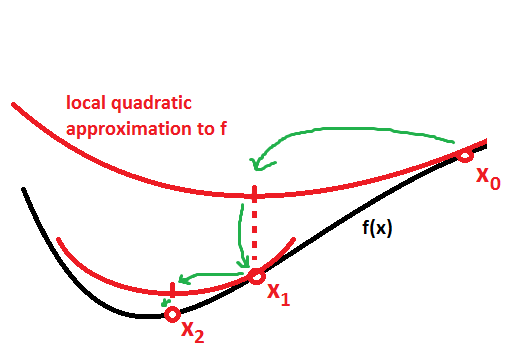
\includegraphics [scale=0.45] {NR-Opt}
\end{center}
In this method, we approximate $f_x$ to be \textbf{quadratic function} at $x_n$ and then try to minimize that function. That point is our new $x_n$.
\end{frame}

\begin{frame}[fragile]{Comparison with Gradient Descent}
 The Gradient Descent Method is a relatively naive approach to solve optimization problems.
 \begin{center}
     $\boldsymbol{x_{n+1}=x_n-\alpha_n*\nabla f(x_n)}$
 \end{center}
 Gradient Descent has \textbf{first order} of convergence while the Newton's Method has \textbf{second order} of convergence.
 \begin{center}
    \graphicspath{ {./images/} }
    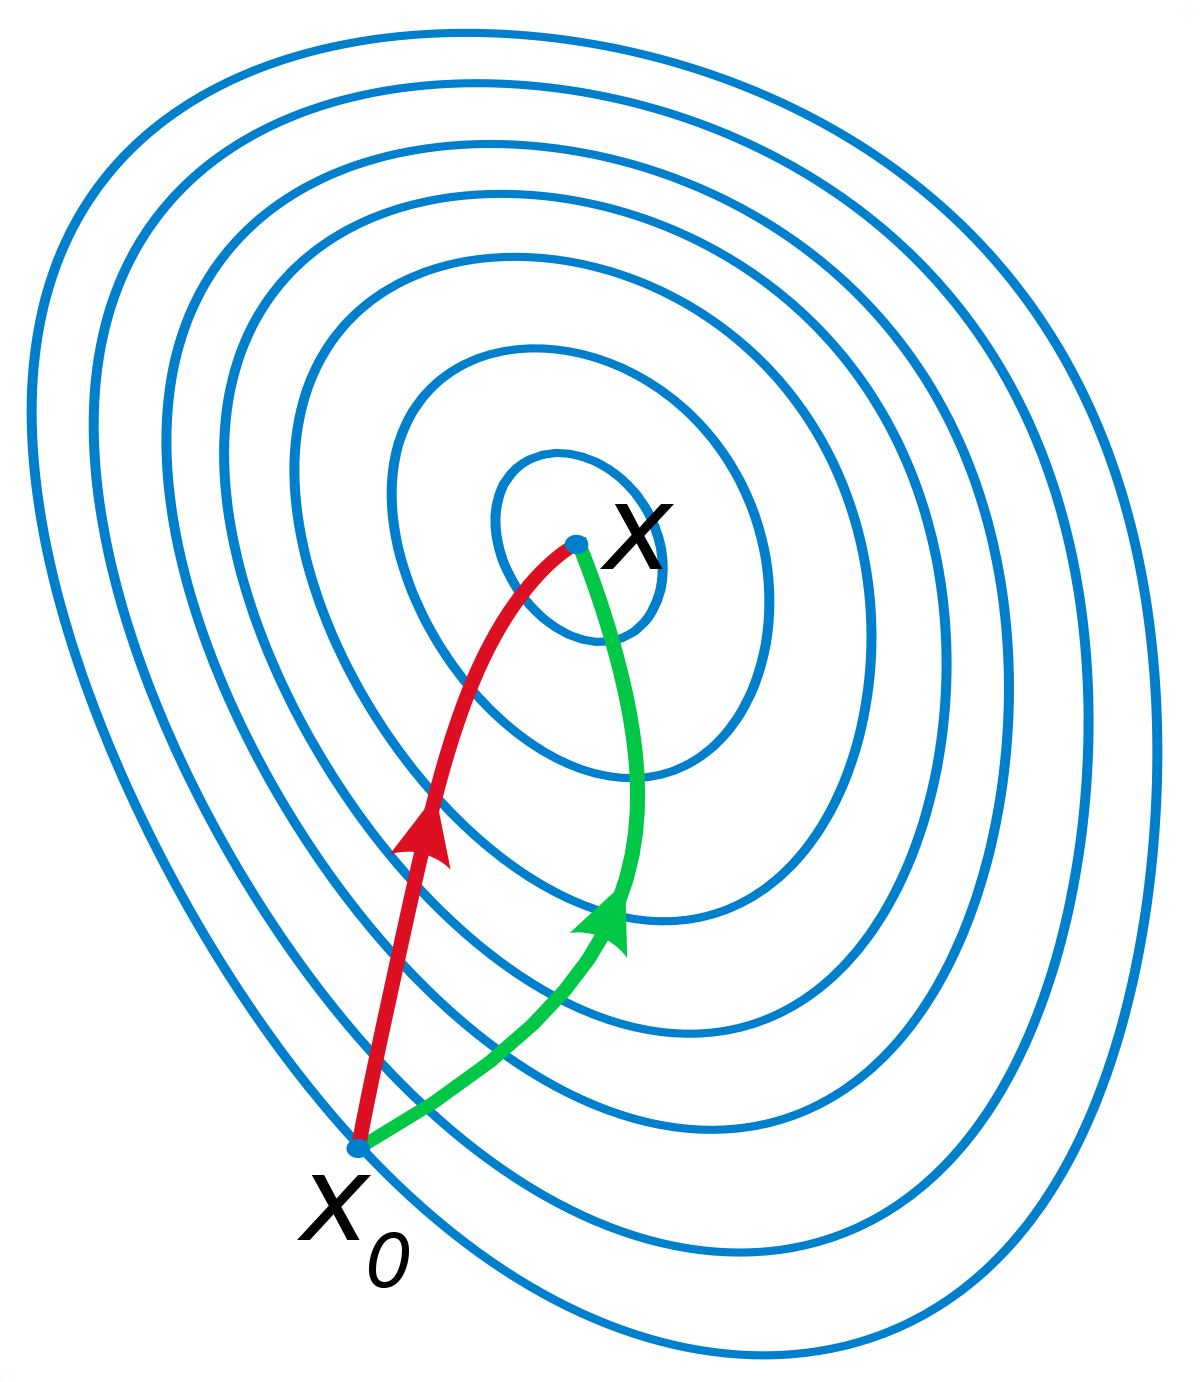
\includegraphics [scale=0.07] {GD}
\end{center}
\begin{center}
A comparison of {\color{green} Gradient Descent} and {\color{red} Newton's Method}.    
\end{center}
\end{frame}

\begin{frame}[fragile]{Newton's Method in Multiple Dimensions}
 \textbf{Idea} : Make a second-order approximation and then minimize that.
 \vspace{2mm}\ \\
 Let $f: \mathbb{R} ^{n} \rightarrow \mathbb{R} $ be sufficiently smooth.
 \vspace{2mm}\ \\
 From \textbf{Taylor's Theorem}, we have \\
 \begin{center}
     $\boldsymbol{f(x) \approx f(a) + g^{T}(x-a) + \frac{1}{2}(x-a)^{T}H(x-a)}$
     \vspace{2mm}\ \\
     where $\boldsymbol{g=\nabla f(a)}$ and $\boldsymbol{H = \nabla ^{2}f(a)}$
 \end{center}
\end{frame}

\begin{frame}[fragile]{Newton's Method in Multiple Dimensions}
 We can rearrange the terms in the Taylor's Theorem to get :
 \begin{center}
     $\boldsymbol{f(x) \approx \frac{1}{2}x^{T}Hx + b^{T}x + c}$
     \vspace{2mm}\ \\
     where $\boldsymbol{b = g - H \cdot a }$ and $\boldsymbol{c = f(a)} $
 \end{center}
 Now, we have to \textbf{minimize} $f(x)$. So, $\nabla f(x) = 0$.
 \begin{center}
     $\boldsymbol{\nabla f(x) = Hx + b =0}$
     \vspace{2mm}\ \\
     $\boldsymbol{\therefore x=-H^{-1}b}$
     \vspace{2mm}\ \\
     $\boldsymbol{\implies x=-H^{-1}(g-H\cdot a)=a-H^{-1}g}$
 \end{center}
 $x$ is a minima only if $\boldsymbol{\nabla ^{2}f(x) \geq 0}$
\vspace{2mm}\ \\
\begin{center}
    $\boldsymbol{\implies \nabla ^{2}f(x) = H \geq 0}$ i.e \textbf{H} must \textbf{positive semi-definite}.
\end{center}
\end{frame}

\begin{frame}[fragile]{Newton's Method in Multiple Dimensions}
 \textbf{Algorithm} :
 \begin{itemize}
     \item Initialize - $\boldsymbol{x_0 \in \mathbb{R}^{n}}$ 
     \vspace{3mm}
     \item Iterate - $\boldsymbol{x_{n+1}=x_n-H^{-1}g}$.
     \vspace{2mm}\ \\
     where $\boldsymbol{g=\nabla f(a)}$ and $\boldsymbol{H = \nabla ^{2}f(a)}$
   \end{itemize}
\textbf{Issues} :
 \vspace{3mm}\ \\
 Inverting the Hessian may not be easy as the dimension increases.
  \vspace{2mm}\ \\
 Rather than finding $\boldsymbol{H^{-1}}$, we can solve for $\boldsymbol{H \cdot y=g}$.
 \vspace{2mm}\ \\
 Now, use the iterative method $\boldsymbol{x_{n+1}=x_n-\alpha_{n}\cdot y}$, where $\boldsymbol{\alpha_{n} > 0}$ is the step size introduced to move faster to the optimum.
\end{frame}

\begin{frame}[fragile]{Affine Invariance of Newton's Method}
 Given $f$, non-singular $A \in \mathbb{R}^{n \times n}$. Let $x=Ay$ and $g(y)=f(Ay)$. Newton steps on $g$ are :
 \begin{center}
     $\boldsymbol{y^{+} = y - \big(\nabla ^{2}g(y)\big)^{-1}\nabla g(y)}$
     \vspace{2mm}\ \\
     $\boldsymbol{y^{+} = y - \big(A^{T}\nabla ^{2}f(Ay)A\big)^{-1}A^{T}\nabla f(Ay)}$
     \vspace{2mm}\ \\
     $\boldsymbol{y^{+} = y - A^{-1}\big(\nabla ^{2}f(Ay)\big)^{-1}\nabla f(Ay)}$
 \end{center}
 Hence,
 \begin{center}
     $\boldsymbol{Ay^{+}=Ay -\big(\nabla ^{2}f(Ay)\big)^{-1}\nabla f(Ay)} $
 \end{center}
 i.e.,
 \begin{center}
     $\boldsymbol{x^{+}=x -\big(\nabla ^{2}f(x)\big)^{-1}\nabla f(x)} $
 \end{center}
 So, we can see that progress is independent of scaling which is why Newton's Method is \textbf{Affine Invariant}. 
\end{frame}

\begin{frame}[fragile]{Newton Decrement}
 At a point $x$ , we define \textbf{Newton Decrement} as 
 \begin{center}
     $\boldsymbol{\lambda(x)=\Big(\nabla f(x)^{T}\big(\nabla^{2}f(x)\big)^{-1}\nabla f(x)\Big)^{1/2}}$
 \end{center}
 This relates to the difference between $f(x)$ and the minimum of it's quadratic approximation:
 \begin{center}
     $\boldsymbol{f(x)-\min\limits_{y}\Big(f(x)+\nabla f(x)^{T}(y-x)+\frac{1}{2}(y-x)^{T}\nabla^{2}f(x)(y-x)\Big)} $
     \vspace{2mm}\ \\
     $\boldsymbol{=f(x)-\Big(f(x)-\frac{1}{2}\nabla f(x)^{T}\big(\nabla^{2}f(x)\big)^{-1}\nabla f(x)\Big)}$
     \vspace{2mm}\ \\
     $\boldsymbol{=\frac{1}{2}\lambda(x)^{2}}$
 \end{center}
 Therefore, we can think of $\frac{1}{2}\lambda(x)^{2}$ as an an approximate upper bound on
the suboptimality gap $\boldsymbol{f(x)-f^{*}}$.`
\end{frame}

\begin{frame}[fragile]{Newton Decrement}
 \textbf{Another Interpretation of Newton Decrement:}
 \vspace{2mm}\ \\
 If Newton's 
 direction/step is $\boldsymbol{v=-\big(\nabla^{2}f(x)\big)^{-1}\nabla f(x)}$ , then 
 \begin{center}
     $\boldsymbol{\lambda(x)=\big(v^{T}\nabla^{2}f(x)v\big)^{1/2}= \left\|v\right\|_{\nabla^{2}f(x)}}$
 \end{center}
 i.e. $\lambda(x)$ is the length of the \textbf{Newton step} in the norm defined by
the Hessian $\boldsymbol{\nabla^{2}f(x)}$.
\end{frame}

\begin{frame}[fragile]{Variants of Newton Methods}
 Let $\alpha$ be a simple zero of a sufficiently differentiable function $f$. 
 \vspace{2mm}\ \\
 \begin{center}
  $\boldsymbol{f(x)=f(x_n) + \mathlarger{\int_{x_n}^{x} f'(t) dt}}$    
 \end{center}
 If we approximate the indefinite integral by the trapezoidal rule and take $x=\alpha$, we obtain
 \begin{center}
     $\boldsymbol{0 \approx f(x_n)+\frac{1}{2}(\alpha-x_n)(f'(x_n)+f'(\alpha))}$
 \end{center}
 So, the new approximation $x_{n+1}$ to $\alpha$ is given by 
 \begin{center}
     $\boldsymbol{x_{n+1}=x_n-\frac{2f(x_n)}{f'(x_n)+f'(x_{n+1})}}$
 \end{center}
 The $(n+1)^{th}$ value of Newton's method is used on the RHS,
 \begin{center}
     $\boldsymbol{x_{n+1}=x_n-\frac{2f(x_n)}{f'(x_n)+f'(z_{n+1})}}$
     \vspace{2mm}\ \\
     where $\boldsymbol{z_{n+1}=x_n-\frac{f(x_n)}{f'(x_n)}}$
 \end{center}
\end{frame}

\begin{frame}[fragile]{Variants of Newton Methods}
 We rewrite the previous equation as
 \begin{center}
  $\boldsymbol{x_{n+1}=x_n-\frac{f(x_n)}{(f'(x_n)+f'(z_{n+1}))/2}}$    
 \end{center}
 So, this variant of Newton's method can be viewed as obtained by using arithmetic mean of $f'(x_n)$
and  $f'(z_{n+1})$ instead of $f'(x_n)$ in Newton's method.
\vspace{2mm}\ \\

Therefore, we call this method \textbf{Arithmetic Mean Newton (AN) Method}. 
\vspace{2mm}\ \\
If we use \textbf{Harmonic Mean} instead of Arithmetic Mean, we get 
\begin{center}
  $\boldsymbol{x_{n+1}=x_n-\frac{f(x_n)\big(f'(x_n)+f'(z_{n+1}\big)}{2f'(x_n)f'(z_{n+1})}}$    
 \end{center}
 which we call as \textbf{Harmonic Mean Newton (HN) Method}.
\end{frame}

\begin{frame}[fragile]{Variants of Newton Methods}
  If we approximate the indefinite integral by the \textbf{mid-point} integration rule, instead of trapezoidal rule and take $x=\alpha$ , we obtain
 \begin{center}
     $\boldsymbol{0 \approx f(x_n)+(\alpha-x_n)f'\big(\frac{x_n+\alpha}{2}\big)}$
 \end{center}
 and in this case a new approximation $x_{n+1}$ to $\alpha$ is given by 
 \begin{center}
     $\boldsymbol{x_{n+1}=x_n-\frac{f(x_n)}{f'\big((x_n+x_{n+1})/2\big)}}$
 \end{center}
 The $(n+1)^{th}$ value of Newton's method is used on the RHS,
 \begin{center}
     $\boldsymbol{x_{n+1}=x_n-\frac{f(x_n)}{f'\big((x_n+z_{n+1})/2\big)}}$
     \vspace{2mm}\ \\
     where $\boldsymbol{z_{n+1}=x_n-\frac{f(x_n)}{f'(x_n)}}$
 \end{center}
 which we call as \textbf{Mid-Point Newton (MN) Method}.
\end{frame}

\begin{frame}[fragile]{Variants of Newton Methods}
  \textbf{Convergence and Numerical Analysis}:
  \begin{itemize}
    \item \textbf{Convergence} : AN, HN, MN methods are \textbf{cubically} convergent while the Classical Newton Methods is \textbf{quadratically} convergent.  
     \item As far as the numerical results are considered, for most of the cases HN method requires the least number of function evaluations while AN and MN methods require almost the same number of function evaluations. 
    
   \end{itemize}
\end{frame}
\begin{frame}{Variants of Newton Methods}
\textbf{Applications} :
 \begin{itemize}
    \item In \textbf{Image Processing} - Image DeBlurring,DeNoising,Plotting Contours etc.,(discussed in detail)
     \item A Combined Newton Method for \textbf{Symmetric Conic Linear Programming}

\item A seventh-order convergent Newton-type method for \textbf{solving nonlinear equations}
\item Newton method for the \textbf{ICA(Independent Component Analysis) mixture model}
\item A Modified Newton Method for \textbf{Unconstrained Convex Optimization}


   \end{itemize}
\end{frame}

\begin{frame}{Variants of Newton Methods}
\textbf{Applications} :
 \begin{itemize}
    
\item An efficient finite-difference-based Newton-Raphson method to determine intrinsic complex \textbf{permeabilities} and \textbf{permittivities} for Mn-Zn ferrites

\item Steady-state calculation of \textbf{electrical power system} by the Newton's Method in optimization

\item Solving \textbf{frictional contact problems} by a semismooth Newton method

\item Truncated Newton Method for \textbf{Solving Minimax Problems}

\item Study of the \textbf{simulation of DC traction power supply} system based on AC/DC unified Newton-Raphson method
     
   \end{itemize}
\end{frame}


\begin{frame}[fragile]{Newton's Method in Image Processing}
 \begin{itemize}
     \item \textbf{Image processing} is a technique which is used to derive information from the images.
     \item Generally used method for solving the cost function is \textbf{Gradient Descent}, which is proper but has lower rate of convergence (linear).
     \item Newton- type methods, on the other hand, are known to have a rapid (quadratic) convergence. In its classical form, the Newton method relies on the \textbf{L2-norm} to define the descent direction. 
    
   \end{itemize}

\end{frame}

\begin{frame}{Newton's Method in Image Processing}
    \begin{itemize}
        \item In report, we generalize and reformulate this very important optimization method by introducing a novel Newton method based on \textbf{general norms}. 
        \item This generalization opens up new possibilities in the extraction of the Newton step, including benefits such as \textbf{mathematical stability} and \textbf{smoothness constraints}. 
    \end{itemize}
\end{frame}
\begin{frame}{Active Contour}
    \begin{itemize}
        \item  \textbf{Segmentation} is a section of image processing for the separation or segregation of information from the \textbf{required target} region of the image. 
        \item There are different techniques used for segmentation of pixels of interest from the image.
        \item \textbf{Active contour} is one of the active models in segmentation techniques, which makes use of the \textbf{energy constraints} and \textbf{forces} in the image for separation of region of interest. 
        \item It defines a separate boundary or curvature for the regions of target object for segmentation
    \end{itemize}
\end{frame}

\begin{frame}{Active Contour}
    \begin{center}
    \graphicspath{ {./images/} }
    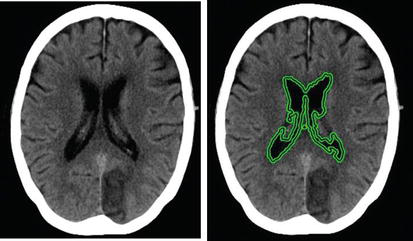
\includegraphics [scale=1] {F1}
\end{center}
\end{frame}

\begin{frame}{Active Contour}
\textbf{Applications} :
 \begin{itemize}
     \item Segmentation of the \textbf{medical images} i.e.,
     \vspace{2mm}
     \item Various medical applications especially for the \textbf{separation of required regions} from the various medical images.
     \vspace{2mm}\ \\
      \item Different types of images from various 3-D imaging modalities like \textbf{MRI}, \textbf{CT}, \textbf{PET}, \textbf{SPECT} scans can be segmented and processed with these active contour models.
   \end{itemize}
\end{frame}

\begin{frame}{References}
\begin{itemize}
    \item \textbf{Convex Optimization by Stephen Boyd.}
    \item \textbf{Newton's Methods and it's Variants.}
     \vspace{1mm}\ \\
    https://www.sciencedirect.com/science/article/pii/S0893965904901048
    \item \textbf{Generalized Newton methods for Energy Formulations in Image Processing.}
     \vspace{1mm} \ \\
            https://ieeexplore.ieee.org/document/4711878
     \vspace{2mm}
     \item \textbf{Image Processing and Active Contour related link.}
     \vspace{1mm}\ \\
     https://www.intechopen.com/books/medical-and-biological-image-analysis/active-contour-based-segmentation-techniques-for-medical-image-analysis
      \end{itemize}
\end{frame}
\end{document}
